\subsection{Destrutor}

A linguagem \acs{PHP} 5, traz consigo o conceito de métodos destrutores de maneira
similar a outras linguagens orientadas a objeto, como o \textit{Java}. Um método
destrutor é um método especial, que na linguagem \acs{PHP} chama-se
\textit{\_\_destruct}, em contrapartida, segundo \citeonline{learningJava}, na
linguagem \textit{Java} o método recebe o nome \textit{finalize}.

Portanto, sempre que um script terminar a sua execução ou quando um objeto for
forçadamente removido, o interpretador irá remover as referências de um objeto
da memória e o método destrutor será executado.

Na Figura \ref{fig:metodoDestrutor}, tem-se a sintaxe da definição de um
método destrutor utilizando a linguagem \acs{PHP}:

\begin{figure}[h!tb]
	\caption{Método destrutor implementado na linguagem PHP}
	\label{fig:metodoDestrutor}

	\centering
	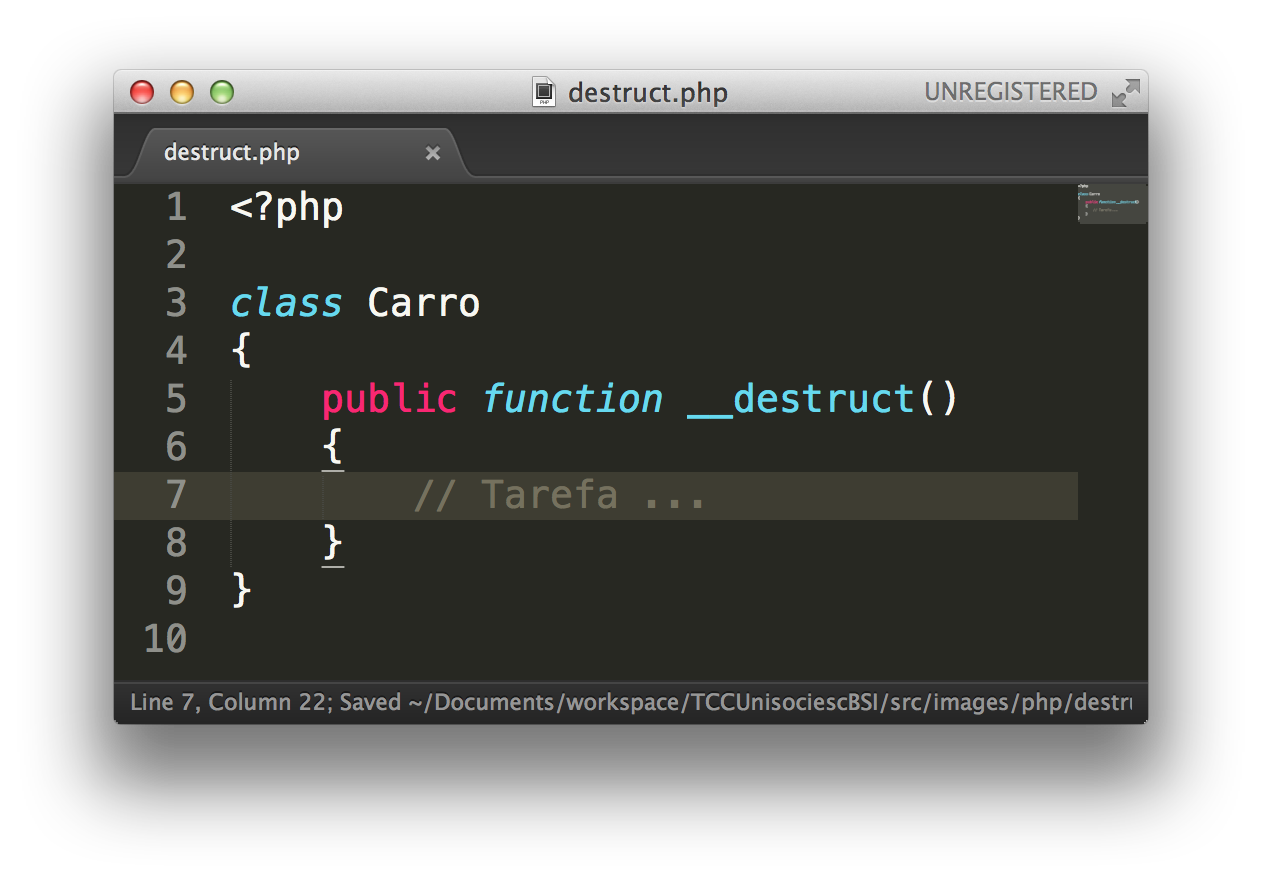
\includegraphics[width=0.75\textwidth]{images/destruct.png}

	\centering
	\footnotesize Fonte: \fonteOAutor
\end{figure}

\FloatBarrier 	% Este comando impede que as imagens
				% flutuem a partir deste ponto no seu documento

A seguir, é apresentado em detalhes as linhas de código exibidas na Figura
\ref{fig:metodoDestrutor}:

\begin{alineas}
    \item linha 5: define-se a existência explícita de um método destrutor;
    \item linha 7: vê-se um comentário da linguagem \acs{PHP} indicando que
    neste local seria executado as funcionalidades do método destrutor, como
    por exemplo a gravação de um arquivo.
\end{alineas}

Em seguida, será definido o conceito de herança.